\documentclass[twoside,english]{uiofysmaster}
%\bibliography{references}

\usepackage{array}
\usepackage{booktabs}
\usepackage{float}
\usepackage{scrextend}
\usepackage{amsfonts}
\usepackage{amsmath,amsfonts,amssymb}
\addtokomafont{labelinglabel}{\sffamily}
\usepackage[compat=1.1.0]{tikz-feynman}
\usepackage{tikz}

\usepackage[boxed]{algorithm2e}
\addtokomafont{labelinglabel}{\sffamily}

% Feynman slash
\usepackage{slashed}

% To show code
\usepackage{listings}

% Multicolumns for calculation
\usepackage{multicol}

% Subfigures
\usepackage{subcaption}
\usepackage{sidecap}

\setlength{\heavyrulewidth}{1.5pt}
\setlength{\abovetopsep}{4pt}

\begin{document}

\tableofcontents

\chapter{Supersymmetry at Hadron Colliders}

At the moment of writing, the Large Hadron Collider (LHC) at CERN is one of the largest and most important particle physics experiments in the world. In this chapter, some of the advantages and challenges of using hadron colliders are discussed, along with some techniques for moving from theory to physically detectable signals. A short description of supersymmetric phenomenology follows, along with current bounds on some supersymmetric particles. Finally, the squark production cross section is calculated to leading order, and next-to-leading order terms are investigated.

\section{Hadron Colliders}

Colliding hadrons makes it possible to reach very high center-of-mass energies. This is owed to the heavy mass scale of hadrons compared to leptons, resulting in low \textit{synchrotron radiation} which makes the use of circular accelerators beneficial. The circular form means the accelerating structures can be reused as many times as one desires, thus putting `no limits' on the energies obtained (there are, of course, limits). Synchrotron radiation is the radiation of energy from a particle being accelerated, which goes as $\sim m^{-4}$. Thus for light particles, such as the electron, a lot of energy is wasted. The power radiated by a relativistic electron forced to move in circular motion with radius $R$ is given by Schwinger's formula \cite{Balerna2015}
\begin{align}
P_e = \frac{2}{3} \frac{e^2 c}{R^2} \Bigg( \frac{E}{m_e c^2} \Bigg)^4,
\end{align}
where $E$ is the electron energy, $m_e$ is the electron mass and $c$ is the speed of light in vacuum. Because the proton mass is much larger than the electron mass, this effect is relatively small, allowing the LHC to operate at energies currently as high as 13 TeV. 

Amidst this praise of the hadron one question arises: if hadronic colliders are able to reach such high energies, why do bother colliding leptons at all? Alas, the heavy masses come at a kinematical price. The way hadrons are made up of valence and sea quarks and gluons make the kinematics of collisions very difficult to calculate. These quarks and gluons, the so-called \textit{partons}, have the annoying habit of distributing the hadron momentum somewhat randomly amongst themselves. Since we do not know how the energy and momentum is distributed, the momenta of the ingoing particles is unknown. This is why the transverse momentum and energy, not to mention the \textit{missing} transverse energy, are important when analysing data from colliders. However, there is a way to approximate the parton momenta, namely using \textit{parton distribution functions}.

\subsection{Parton Distribution Functions}

Cross sections are calculated for two colliding partons, for example two quarks $q_1 q_2$. The cross section is a function of the center-of-mass energy, $\hat{s}$, which again can be written as a fraction of the center of mass of the colliding protons
\begin{align}
\hat{s} = s x_1 x_2,
\end{align}
where $s$ is the center-of-mass energy of the colliding protons, and $x_i$ is the momentum fraction of the quark $q_i$. The fractions of momenta are then integrated over, using \textit{parton distribution functions} $f(x_i)$, which differ for the different partons. The fraction $x_u$ for an up-type quark in a proton e.g., would be much larger than that for a top-type squark. This yields the total cross section
\begin{align}
\sigma_{q_1q_2} = \int f(x_1) f(x_2) \sigma(\hat{s}) dx_1 dx_2,
\end{align}
where $\sigma$ is the partonic cross section. In this project the CTEQ6 parton distribution functions from the LHAPDF Fortran library \cite{PhysRevD.78.013004}.

\subsection{Luminosity}

Another important concept to be introduced is \textit{luminosity}. The luminosity $\mathcal{L}$ is a measure on how many collisions happen at an accelerator per time, and is here given in inverse femto-barn $\text{fb}^{-1} = 10^{43} \text{ m}^{-2}$. This can be used to set limits on the size of cross section, by considering the following relation for a process where a particle $A$ is produced
\begin{align}
n_{A} = \mathcal{L} \sigma_{A} ,
\end{align}
where $\mathcal{L}$ is the luminosity, $\sigma_{A}$ is the cross section for the production of $A$, and $n_A$ is the number of produced particles. Setting $n=1$ as the limit for a single produced particle, and using $\mathcal{L} = 20.3 \text{ fb}^{-1}$, which is the luminosity for the dataset used here, the lower limit on cross sections is
\begin{align}
\sigma  = \frac{1}{20.3 \text{ fb}^{-1}} \approx 0.05 \text{ fb}.
\end{align}
Therefore, cross sections below $\sigma \sim \mathcal{O}(10^{-3})$, which correspond $0.02$ produced particles, will be less important in this thesis.


\section{Phenomenology}
In order to know what to look for at the LHC it is necessary to consider the phenomenology of supersymmetry. This is done by first revisiting the soft supersymmetry breaking, in order to consider models with more constraints than the 124 parameters of the MSSM. \textit{Hidden sector} (HS) scalar superfields $X$ have very small or no interactions with the MSSM fields. Their couplings are usually supressed by some mass scale so that $\mathcal{L} \sim M^{-1}$. They have an effective (non-renormalizable) interaction  with the scalar superfields of the form
\begin{align}
\mathcal{L}_{HS} &= - \frac{1}{M} (\bar{\theta} \bar{\theta}) X \Phi_i \Phi_j \Phi_k.
\end{align}
If these sectors develope a vacuum expectation value $\braket{X} = \theta \theta\braket{F_X}$ for the auxilliary field $F$ (auxilliary meaning that it can be removed using the Euler-Lagrange equations),  supersymmetry is broken. The two most commonly known hidden sectors are Planck-scale mediated supersymmetry breaking (PMSB) and Gauge mediated supersymmetry breaking (GMSB), the first of which is obtained by blaming some gravity mechanism for mediating the breaking of SUSY from the hidden sector. The breaking scale is then the Plank scale, $M = M_P = 2.4 \cdot 10^{18}$ GeV. The vev is restricted to $\sqrt{\braket{F}} \sim 10^{10} - 10^{11}$ GeV in order not to reintroduce the hierarchy problem.  The complete soft terms can be shown to be \cite{batzing2017lecture}
\begin{align*}
\mathcal{L}_{soft} =& - \frac{\braket{F_X}}{M_P} \Big( \frac{1}{2} f_a \lambda^a \lambda^a + \frac{1}{6} y_{ijk}'A_i A_j A_k + \frac{1}{2} \mu_{ij}' A_i A_j + \frac{\braket{F_X}^*}{M_P^2}  x_{ijk} A_i^* A_j A_k + c.c.\Big)\\
&- \frac{|\braket{F_X}|^2}{M_P} k_{ij}A_i A_j^*.
\end{align*}
By simplifying as much as possible, all soft terms are fixed by just four parameters. This model is called minimal supergravity (mSUGRA) or the constrained minimal supersymmetric Standard Model (CMSSM). The CMSSM parameters are
\begin{align}
&m_{1/2} = f \frac{\braket{F_X}}{M_P}, & m_0^2 = k \frac{|\braket{F_X}|}{M_P^2}, 
&& A_0 = \alpha \frac{\braket{F_X}}{M_P}, &&B_0 = \beta \frac{\braket{F_X}}{M_P},
\end{align}
or $m_{1/2}$, $m_0$, $A_0$, $\tan \beta$ and $\text{sgn} \mu$.

The second hidden sector is the aforementioned Gauge mediated supersymmetry breaking. In this case the soft terms come from loop diagrams with \textit{messenger superfields} that get their own mass from coupling to the HS SUSY breaking vev, and have SM interactions. This model is parameterized by 
\begin{align}
\Lambda = \frac{\braket{F}}{M_{messenger}} \text{ , } M_{messenger} \text{ , } N_5 \text{ , } \tan \beta,
\end{align}
where $M_{messenger}$ is the mass scale and $N_5$ (FYLL INN HER).

\subsection{Searches For Supersymmetry}

Supersymmetry at hadron colliders will be in the form of QCD processes with relatively small masses, as the incoming particles are quarks and gluons and QCD cross sections will therefore be the largest. The traces left by such processes will be closely related to the conservation of $R$-parity, in that all sparticles are produced in pairs and eventually decay to the LSP. If the LSP is indeed only weakly interacting, this makes it very difficult to detect. An indirect way of detecting it, however, is by looking for \textit{missing transverse energy} $\slashed{E}_T$. The energy is only considered in the transverse plane, as the longitudinal momentum is difficult to predict in the hadronic case (see the above discussion of hadron colliders). To look for $\slashed{E}_T$ the \textit{effective mass} is defined as
\begin{align}
M_{eff} &= \sum p_T^{jet} + \slashed{E}_T,
\end{align} 
and used to search for deviations from the SM expectations. Here $p_T^{jet}$ is the transverse momentum of jets. The hadronic jets produced from supersymmetric processes can be very complicated, such as the squark-squark production shown in Fig. (\ref{Fig:: susy hadron : decay at ATLAS}). If all final state particles have low momenta, these are called soft particles. The very large background from SM processes provides another difficulty in searching for supersymmetry. An example generated with ATLAS Open Data is shown in Fig. (\ref{Fig:: susy hadron : ATLAS susy analysis}), where the supersymmetric signals (pink lines) are all below the SM background, and so it is impossible to detect any deviation from SM background. 

\begin{figure}[H]
\centering
\begin{tikzpicture}
\begin{feynman}
\vertex (p1) {\(p\)}; 
\vertex [below right=of p1, blob] (p) {}; 
\vertex [below left=of p] (p2){\(p\)}; 
%----------------------------------
\vertex [right=1.5cm of p] (mid1);\vertex [above=0.7cm of mid1] (s1);
\vertex [below =0.7cm of mid1] (s2);
\vertex [right=1.5cm of s1] (q1); 
\vertex [right=1.5cm of s2] (q2) ; 
%---------------------------------
\vertex [right=1cm of q1] (r1) ; %W
\vertex [right=1cm of q2] (r2) ; %W
%--------------------------------
\vertex [right=1cm of r1] (rl) {\(l\)};
\vertex [above=0.7cm of rl] (rn) {\(\nu\)};
\vertex [right=1cm of r2] (rq1) {\(q\)};
\vertex [below=0.7cm of rq1] (rq2) {\(q\)};
%--------------------------------
\vertex [above=0.7cm of rn] (r11) {\(\tilde{\chi}_1^0\)};
\vertex [below=0.7cm of rq2] (r22) {\(\tilde{\chi}_1^0\)};
\vertex [above=0.7cm of r11] (q11) {\(q\)}; 
\vertex [below=0.7cm of r22] (q22) {\(q\)};
\diagram{
(p1)--(p)--(p2), 
(p) --[scalar, edge label={\(\tilde{q}\)}] (s1), 
(s2) --[scalar, edge label={\(\tilde{q}\)}] (p); 
(q1) --[photon, plain, edge label= {\(\tilde{\chi}_1^{\pm}\)}, ] (s1); 
(s1) -- (q11); (s2) --[photon, plain, edge label= {\(\tilde{\chi}_1^{\pm}\)}] (q2); 
(s2) -- (q22), 
(r1) -- [photon, edge label={\(W\)}] (q1),
 (q1) --[photon, plain](r11), 
 (q2) --[photon, edge label={\(W\)}] (r2), 
 (q2) --[photon, plain] (r22),
(rn)--(r1) -- (rl), 
(rq1) -- (r2) -- (rq2)
};
\end{feynman}
\end{tikzpicture}
\caption{Possible signature of a supersymmetric QCD process, with four quark jets, a lepton and large missing transverse energy in the final state.}
\label{Fig:: susy hadron : decay at ATLAS}
\end{figure}

\begin{figure}
\centering
\includegraphics[scale=0.5]{Figures/mt_rebinned.pdf}
\caption{Analysis of ATLAS data, where the pink lines are supersymmetric signals for $m_{\tilde{q}}=500$ (magenta), $m_{\tilde{q}}=900$ (light pink) and $m_{\tilde{q}}=1100$ (purple). The signal never exceeds the SM background, in this case Diboson (orange), Drell Yan (light blue), $W$ (dark orange), $Z$ (dark blue), $\tilde{t}$ (yellow) and $t \bar{t}$ (green), making it impossible to distinguish events from background. Analysis using $1 \text{ fb}^{-1}$. }
\label{Fig:: susy hadron : ATLAS susy analysis}
\end{figure}

Allowing the violation of R-parity opens up for more possibilities. Then the LSP can decay, and sparticles can be produced one at a time. It is possible to have \textit{massive metastable charged particles} (MMCPs), which are typical for scenarios with a gravitino LSP \cite{batzing2017lecture}.



\subsection{Current Bounds on Sparticles}

Searches and limits are constantly being updated, but here are a few results from the LHC Run I at 8 TeV, with up to $20 \text{ fb}^{-1}$ luminosity. The bounds from the missing energy channel at 8 TeV for mSUGRA from ATLAS are $m_{\tilde{q}} > 1600$ GeV and $m_{\tilde{g}} > 1100$ GeV \cite{batzing2017lecture}.

%\subsection{Precision Observables}

%We can also measure SUSY by considering its impact on very precisey measured SM processes, such as electroweak precision observables, the $(g-2)_{\mu}$ value, the flavour changing neutral current (FCNC) process $b \rightarrow s \gamma$ and the (rare) FCNC process $B_s \rightarrow \mu \mu$.
%
%The electroweak precision observables include $M_W$, $M_Z$, $\Gamma_W$, $\Gamma_Z$, $m_t$ and $\sin \theta_W$, the higgs mass $m_h$ and its properties. Since the Higgs has been measured, we can now do very precise measurements of these quantities, and find that they are very consistent with SM predictions.
%
%The anomalous magnetic moment of the muon, $(g - 2)_{\mu}$, has been measured to extraordinary precision at BNL to be
%\begin{align*}
%g_{\mu} = 2.00116592089(63),
%\end{align*}
%where the digits in parenthesis indicate the uncertainty on the last digits. At tree level we have $\mu \rightarrow \mu \gamma$. Loop corrections to this diagram give $a_{\mu} = (g -2)_{\mu}$. The difference between the SM deviation and the experimentally measured deviation is
%\begin{align*}
%\delta_{a_{\mu}} \equiv a_{\mu}^{exp} - a_{\mu}^{SM}= (25.9 \pm 8.1) \cdot 10^{-10},
%\end{align*}
%which is $3.2 \sigma$ away from zero. This is one of the clearest discrepancies that exist between measurement and the SM.


\section{Squark-Squark Cross Section}
In this thesis the relevant QCD process will be the production of squark pairs in quark-quark collisions,
\begin{align}
q_i q_j \rightarrow \tilde{q}_i \tilde{q}_j,
\end{align}
where $i,j$ are the 4 light quark flavours $u, d, s, c$ which can be equal or different. Top and bottom are not considered here because of their large masses. Feynman diagrams of the leading order for this process can be found in Fig. (\ref{Fig:: susy hadron : Feynman qq}). For equal flavour quarks there are two diagrams contributing: the $t$- and $u$-channel, while for different flavours only the $t$-channel contributes.

\begin{figure}
\centering
\begin{tikzpicture}
\begin{feynman}
\vertex (p1) {\(q_i\)}; \vertex [right= of p1] (s1); \vertex [right= of s1] (q1){\(\tilde{q}_i\)}; \vertex [below=of p1] (p2) {\(q_j\)}; \vertex [right=of p2] (s2) ; \vertex [right= of s2] (q2) {\(\tilde{q}_j\)} ;
\diagram{
(p1) --[fermion, momentum=\(k_1\)] (s1) -- [scalar, momentum=\(p_1\)] (q1), (s1)-- [gluon] (s2) -- (s1), (p2) --[fermion, momentum=\(k_2\)] (s2) --[scalar, momentum=\(p_2\)] (q2)
};
\end{feynman}
\end{tikzpicture}
\begin{tikzpicture}
\begin{feynman}
\vertex (p1) {\(q_i\)}; \vertex [right= of p1] (s1); \vertex [right= of s1] (q1){\(\tilde{q}_i\)}; \vertex [below=of p1] (p2) {\(q_j\)}; \vertex [right=of p2] (s2) ; \vertex [right= of s2] (q2) {\(\tilde{q}_j\)} ;
\diagram{
(p1) --[fermion] (s1) -- [scalar] (q2), (s1)-- [gluon] (s2) -- (s1), (p2) --[fermion] (s2) --[scalar] (q1)
};
\end{feynman}
\end{tikzpicture}
\caption{Feynman diagrams for squark pair production in quark quark collisions, both $t$ and $u$ diagram. Note that the u-channel (right diagram) is only possible for $i=j$.}
\label{Fig:: susy hadron : Feynman qq}
\end{figure}


%\subsection{Feynman Diagrams}

\subsection{Calculation to LO}

The cross section for squark production is here calculated to leading order. The momentum of the gluino is denoted $p$ in the calculations, and defined as $p= k_2-p_2 $ for the $t$-channel and $p=k_2-p_1$ for the $u$-channel. The chiralitites are decided later, and are simply denoted as $P$ and $P'$ for now. The Feynman gauge is used, and all quark masses are set to zero. A more detailed calculation can be found in Appendix A. The expression for the matrix element of the pure $t$-channel becomes (reading direction is from $q_j$ to $q_i$)
\begin{align*}
i \mathcal{M} &= \bar{v} (k_1) \Big( -i \sqrt{2} g P (t_a)^{ij}\Big) \times \delta^{ab} \frac{i}{\slashed{p} - m_{\tilde{g}}} \times \Big( -i \sqrt{2} gP'(t_b)^{lk} \Big) \times u(k_2)\\
&= - \frac{i 2 g^2}{p^2 - m_{\tilde{g}}^2 + i \epsilon}\big( \bar{v} (k_1)  P (t_a)^{ij}(\slashed{p} + m_{\tilde{g}}) P'(t^a)^{lk} u(k_2) \big)\\
&= - (t_a)^{ij}(t^a)^{lk} \times \frac{i 2 g^2}{t_g^2} \times  \bar{v} (k_1)  P (\slashed{p} + m_{\tilde{g}}) P' u(k_2) ,
\end{align*}
where the color factor has been factored out. The charge conjugate matrix element
\begin{align*}
i \mathcal{\bar{M}} & = (t_a)^{ij}(t^a)^{lk} \times \frac{i 2 g^2}{t_g^2} \times \bar{u} (k_2)  P (\slashed{p} + m_{\tilde{g}}) P' v(k_1) .
\end{align*}
Some Mandelstam variables have been used to clean up the expresson; $t= p^2 = (k_2 - p_2)^2$, $t_g = t - m_{\tilde{g}}^2$. The matrix element squared is then
\begin{align*}
|\mathcal{M}_t|^2 &=  (t_a)^{ij} (t^a)^{lk} (t_b)^{mn} (t^b)^{op} \times \frac{4 g^4}{t_g^2}
\big( \bar{v} (k_1)  P (\slashed{p} + m_{\tilde{g}}) P' u(k_2) \big)
\big( \bar{u} (k_2)  P (\slashed{p} + m_{\tilde{g}}) P' v(k_1) \big)
\end{align*}
Now average over spin
\begin{align*}
\sum |\mathcal{M}|^2 &= A_{color, t} \times \frac{4 g^4}{t_g^2} \text{tr} \big[ 
\slashed{k}_1 P (\slashed{p} + m_{\tilde{g}}) P' \slashed{k}_2 P (\slashed{p} + m_{\tilde{g}}) P' \big],
\end{align*}
where $A_{color, t}= (t_a)^{ij} (t^a)^{lk} (t_b)^{mn} (t^b)^{op}$. Since the quark mass is small compared to $m_g$, $m_{\tilde{q}}$ and $m_{\tilde{g}}$, we've set $m_q=0$.
Consider the different combinations of chiralities whose traces are
\begin{center}
\textit{Different chiralities }$P=P_{R/L}$, $P'=P_{L/R}$
\end{center}
\begin{align}\label{Eq:: susy hadron : calc chiralities}
\text{tr} \big[ 
\slashed{k}_1 P_{R/L} (\slashed{p} + m_{\tilde{g}}) P_{L/R} \slashed{k}_2 P_{R/L} (\slashed{p} + m_{\tilde{g}}) P_{L/R} \big]
&= 2 \big(
2 (p \cdot k_2) (k_1 \cdot p) - p^2 (k_1 \cdot k_2)\big).
\end{align}

\begin{center}
\textit{Equal chiralities} $P=P_{R/L}$, $P'=P_{R/L}$
\end{center}
\begin{align*}
\text{tr} \big[ 
\slashed{k}_1 P_{R/L} (\slashed{p} + m_{\tilde{g}}) P_{R/L} \slashed{k}_2 P_{R/L} (\slashed{p} + m_{\tilde{g}}) P_{R/L} \big]&= 2  m_{\tilde{g}}^2 (k_1 \cdot k_2)
\end{align*}
where $P_{R/L}P_{R/L} = P_{R/L}$, $(\gamma^5)^2 = 1$ and $\text{tr}[\gamma^5 \gamma^{\mu} \gamma^{\nu}]=0$. In terms of the Mandelstam variables, here defined as
\begin{multicols}{3}

\begin{align*}
s &= (k_1 + k_2)^2 = 2 k_1 \cdot k_2\\
t &= (k_2-p_2)^2 = m_{\tilde{q}}^2 - 2 (k_2 \cdot p_2),\\
u &= (k_1 - p_2)^2 = m_{\tilde{q}}^2 - 2 (k_1 \cdot p_2),
\end{align*}

\begin{align*}
t_1 &= (k_2-p_2)^2 - m_{\tilde{q}}^2,\\
u_1 &= (k_1-p_2)^2 - m_{\tilde{q}}^2,
\end{align*}

\begin{align*}
t_g &= (k_2-p_2)^2 - m_{\tilde{g}}^2,\\
u_g &= (k_1-p_2)^2 - m_{\tilde{g}}^2,
\end{align*}

\end{multicols}
the expression in (\ref{Eq:: susy hadron : calc chiralities}) is simplified to
\begin{align*}
&2(2 (p \cdot k_2) (k_1 \cdot p) - p^2 (k_1 \cdot k_2) ) + 2m_{\tilde{g}}^2 (k_1 \cdot k_2) =  2 \big[t_1u_1 -s(m_{\tilde{q}}^2 - m_{\tilde{g}}^2) \big].
\end{align*}
Note that for equal quark flavors, the two possibilities for different chiralities are in fact equal, and so there should be a factor of $1/2$ there, which yields 
\begin{align*}
\sum |\mathcal{M}|^2 =&   (t_a)^{ij} (t^a)^{lk} (t_b)^{mn} (t^b)^{op}  \times\frac{4 g^4}{t_g^2} \Big[\delta_{ij} \big(\frac{1}{2}(t_1u_1 -sm_{\tilde{q}}^2)+  sm_{\tilde{g}}^2 \big)\\& + (1-\delta_{ij})\big(t_1u_1 -s(m_{\tilde{q}}^2- m_{\tilde{g}}^2) \big)\Big].
\end{align*}
The color factor is
\begin{align*}
(t^a)^{ij}(t_a)^{kl}(t^b)_{ij}(t_b)^{kl} = \frac{1}{2}NC_F,
\end{align*}
where $C_F = \frac{N^2 -1}{2}$. Adding a factor $2$ because of the sum over different chiralities, the full expression for the $t$-channel is
\begin{align*}
\sum |\mathcal{M}_t|^2 &= NC_F \frac{4g^4}{t_g^2} \Big[ \delta_{ij} \big(\frac{1}{2}(t_1u_1-sm_{\tilde{q}}^2) + sm_{\tilde{g}}^2 \big) + (1-\delta_{ij}) \big(t_1u_s - s(m_{\tilde{q}}^2 - m_{\tilde{g}}^2) \big)\Big]
\end{align*}

The expression for the $u$-channel diagram is identical, except the exchange of $t_g^2 \rightarrow u_g^2$, and it only contributes for $i =j$, so the matrix element is
\begin{align*}
\sum |\mathcal{M}_u|^2 &= \delta_{ij} NC_F \frac{4g^4}{u_g^2} \Big[ \frac{1}{2}(t_1u_1-sm_{\tilde{q}}^2) + sm_{\tilde{g}}^2 \Big]. 
\end{align*}


\subsection*{Cross term}
The $ut$ cross term has the matrix element
\begin{align*}
i \mathcal{M}_{ut} &= A_{color, ut}\frac{-i 2 g^2}{t_g}\big( \bar{v} (k_1)  P (\slashed{p} + m_{\tilde{g}}) P'u(k_2) \big)  \frac{i 2 g^2}{u_g} \big( \bar{u} (k_2)  P (\slashed{p} + m_{\tilde{g}}) P' v(k_1) \big)\\
\sum \mathcal{M}_{ut} &= A_{color, ut} \frac{4 g^4}{u_gt_g}\big( \slashed{k}_1   P (\slashed{k}_2 - \slashed{p}_2 + m_{\tilde{g}}) P'\slashed{k}_2  P (\slashed{k}_2 -\slashed{p}_1 + m_{\tilde{g}}) P' \big)\\
\end{align*}
Average over spins
\begin{align*}
\sum  \mathcal{M}_{ut} 
  &= \delta_{ij} A_{color, ut} \frac{4 g^4}{u_gt_g} \big(
  -   t_1 u_1 + m_{\tilde{q}}^2 s 
+  m_{\tilde{g}}^2 s
  \big)\\
\end{align*}
The other cross term --  $tu$ -- is similar, but yields a slightly different combination
\begin{align*}
\sum i \mathcal{M}_{tu} 
  &= \delta_{ij} A_{color, ut} \frac{4 g^4}{u_gt_g} \big(
u_1t_1- m_{\tilde{q}}^2s + m_{\tilde{g}}^2s
  \big).
\end{align*}
Adding the cross terms and summing over the possible chiralities $P_RP_R$ and $P_LP_L$ then gives 
\begin{align*}
\sum |\mathcal{M}_{ut+tu}| &= \delta_{ij} A_{color, ut} \frac{8 g^4}{u_gt_g} \big(2 m_{\tilde{g}}^2s   \big).
\end{align*}
The color factor is
\begin{align*}
\sum_{a,b}(t^a)^{ij}(t_a)^{kl}(t^b)_{ik}(t_b)_{jl} 
 &= - \frac{1}{2}C_F.
\end{align*}



Combination of the matrix elements gives
\begin{align*}
\sum |\mathcal{M}|^2 =& \delta_{ij}  \Bigg[2 g^4NC_F(u_1t_1-sm_{\tilde{q}}^2) \big( \frac{1}{t_g^2} + \frac{1}{u_g^2} \big) + 4 g^4 sm_{\tilde{g}}^2 \Big( NC_F \big(\frac{1}{t_g^2} + \frac{1}{u_g^2}\big) -2C_F\frac{1}{u_gt_g} \Big) \Bigg]\\
&+ (1-\delta_{ij})\Bigg[4g^4NC_F  \frac{u_1t_1-s(m_{\tilde{g}}^2-m_{\tilde{g}}^2)}{t_g^2} \Bigg].
\end{align*}


\subsection*{Cross section}

The cross section for the process $q_iq_j \rightarrow \tilde{q}_i \tilde{q}_j$ is \cite{beenakker1997squark}
\begin{align*}
\sigma^B &= \frac{\pi \alpha_s^2}{s} \Bigg[\beta_{\tilde{q}} \Big(-\frac{4}{9} - \frac{4m_-^4}{9(m_{\tilde{g}}^2s+m_-^4)} \Big) + \Big(-\frac{4}{9}- \frac{8m_-^2}{9s} \Big) L_1 \Bigg]
+ \delta_{ij} \frac{\pi \alpha_s^2}{s} \Bigg[ \frac{8m_{\tilde{g}}^2}{27(s+2m_-^2)} L_1 \Bigg],
\end{align*}
where
\begin{align*}
&L_1 = \ln \Big( \frac{s+2m_-^2-s \beta_{\tilde{q}}}{s+ 2m_-^2+s \beta_{\tilde{q}}} \Big), &\beta_{\tilde{q}} = \sqrt{1-\frac{4m_{\tilde{q}}^2}{s}}, &&m_-^2 = m_{\tilde{g}}^2 - m_{\tilde{q}}^2, &&\alpha_s = \frac{g_s^2}{4 \pi}.
\end{align*}

\section{NLO Corrections}

The next-to-leading order terms contain virtual corrections to the Born level (tree-level) Feynman digrams. By allowing more complicated feynman diagrams, virtual particles can appear in the process. These never make it to the final state and become real particles, but are in stead absorbed by the process. Since they are never real, or on-shell, they can have any momentum and mass. Thus, it is necessary to integrate over all possible momenta, which leads to divergences and infinities. There are three main categories of divergences, namely ultraviolate, infrared and collinear. Ultraviolet divergences appear when the integral is over an energy without bounds, thereby adding infinities. When the inverse problem occurs, that low momentum gives infinities, this is called an infrared divergence. Collinear divergences are also called mass singularities, and stem from exactly that -- masses going to zero.

\begin{figure}
    \centering
    \begin{subfigure}[b]{0.8\textwidth}
        \begin{tikzpicture}
\begin{feynman}
\vertex (p1); \vertex [right= 1cm of p1, blob] (s1) {}; \vertex [right=1.4cm of s1] (q1);
\diagram{
(p1) -- (s1) , (p1) -- [gluon]  (s1), (q1) -- (s1) -- [gluon] (q1)
};

\hspace{3.3 cm}
\node {=};
\hspace{0.3 cm}

\vertex (p2); \vertex [right= 1cm of p2] (s2); \vertex [right=1cm of s2] (q2); \vertex [right = 1cm of q2] (r2);
\diagram{
(p2) -- (s2) -- [gluon, half right] (q2), (p2) -- [gluon]  (s2),(q2)-- [gluon, half right] (s2) -- [half left] (q2), (q2) -- [gluon] (r2) -- (q2)
};

\hspace{3.3 cm}
\node {+};
\hspace{0.3 cm}

\diagram{
(p2) -- (s2) -- [fermion, half right] (q2), (p2) -- [gluon]  (s2),(q2)-- [scalar, half right] (s2), (q2) -- [gluon] (r2) -- (q2)
};
\hspace{3.3 cm}
\node {+};
\hspace{0.3 cm}
\diagram{
(p2) -- (s2),(q2) -- [fermion, half right] (s2), (p2) -- [gluon]  (s2),(s2)-- [scalar, half right] (q2), (q2) -- [gluon] (r2) -- (q2)
};
\end{feynman}
\end{tikzpicture}
        \caption{Gluino self-energy.}
        \label{fig:gull}
    \end{subfigure}
    ~ %add desired spacing between images, e. g. ~, \quad, \qquad, \hfill etc. 
      %(or a blank line to force the subfigure onto a new line)
    \begin{subfigure}[b]{0.8\textwidth}
        \begin{tikzpicture}
\begin{feynman}
\vertex (p1); \vertex [right = 1 cm of p1, blob] (s1) {}; \vertex [above right= 1 cm of s1] (q1); \vertex [below right = 1cm of s1] (r1);
\diagram{
(p1) -- [fermion] (s1), (s1) -- [gluon] (r1) -- (s1), (s1) -- [scalar] (q1)
};

\hspace{2.5 cm}
\node {=};
\hspace{0.3 cm}

\vertex (p2); \vertex [right = 1 cm of p2] (s2); \vertex at (2.0,0.4) (q2); \vertex at (2.5, 0.7) (q22); \vertex at (2.0,- 0.4) (r2); \vertex at (2.5, -0.7) (r22);
\diagram{
(p2) -- [fermion] (s2); (s2) -- [scalar] (q2) -- [scalar] (q22); (s2) -- [gluon] (r2) -- [gluon] (r22), (s2) -- (r2) -- (r22), (r2) -- [gluon] (q2)
};

\hspace{2.7 cm}
\node {+};
\hspace{0.3 cm}

\diagram{
(p2) -- [fermion] (s2); (s2) -- [fermion] (q2) -- [scalar] (q22); (s2) -- [gluon] (r2) -- [gluon] (r22), (r2)-- (r22), (r2) -- [gluon] (q2), (r2) -- (q2)
};

\hspace{2.7 cm}
\node {+};
\hspace{0.3 cm}

\diagram{
(p2) -- [fermion] (s2), 
(q2) -- [scalar] (q22),
(r2) -- [gluon] (r22) -- (r2), 
(s2) -- [fermion] (r2),
(s2) -- [gluon] (q2),
(r2) -- [scalar] (q2)
};

\hspace{2.7 cm}
\node {+};
\hspace{0.3 cm}

\diagram{
(p2) -- [fermion] (s2), 
(q2) -- [scalar] (q22),
(r2) -- [gluon] (r22) -- (r2), 
(s2) -- [scalar] (r2),
(s2) -- [gluon] (q2) -- (s2),
(r2) -- [fermion] (q2)
};

\end{feynman}
\end{tikzpicture}
        \caption{Quark-squark-gluino coupling.}
        \label{fig:tiger}
    \end{subfigure}
    ~ %add desired spacing between images, e. g. ~, \quad, \qquad, \hfill etc. 
    %(or a blank line to force the subfigure onto a new line)
    \begin{subfigure}[b]{0.8\textwidth}
    	\centering
        \begin{tikzpicture}
\begin{feynman}
\vertex at (0,-1) (p1); \vertex at (0,1) (p2); \vertex at (0.5,-0.5) (s1); \vertex at (0.5, 0.5) (s2); \vertex at (1.5,-0.5) (q1); \vertex at (1.5,0.5) (q2); \vertex at (2,-1) (r1); \vertex at (2, 1) (r2);

\diagram{
(p1) -- [fermion] (s1) --[scalar] (q1) --[scalar] (r1);
(p2) -- [fermion] (s2) --[scalar] (q2) --[scalar] (r2);
(s1) --[gluon] (s2) -- (s1);
(q1) --[gluon] (q2)
};
\end{feynman}
\end{tikzpicture}
        \caption{Box diagram.}
        \label{fig:mouse}
    \end{subfigure}
    \caption{A selected set of Feynman diagrams for the virtual corrections of $q_iq_j \rightarrow \tilde{q}_i \tilde{q}_j$ \cite{beenakker1997squark}.}
\label{Fig:: hadron susy : virtual correction Feynman diagrams}
\end{figure}



Including these corrections means integrating out the divergences using dimensional regularization, and sometimes renormalizing parameters. Renormalizing a parameter means giving it a scale dependence, and baking the infinities into this expression. Physically, this means that for example the electromagnetic coupling becomes stronger the closer to a charged particle you get (higher energy). These calulations are often very complicated and tedious.

So, why should we calculate these cumbersome NLO terms? Firstly, the leading order terms are highly dependent on the a priori unknown renormalization scale, leading to a large uncertainty in theoretical predictions (up to a factor of two). Adding higher order terms reduces the scale dependency. Secondly, the NLO contributions are expected to be large and positive, thereby raising the cross sections significantly and allowing for higher bounds on the gluino and squark masses \cite{beenakker1997squark}.

\begin{figure}
\centering
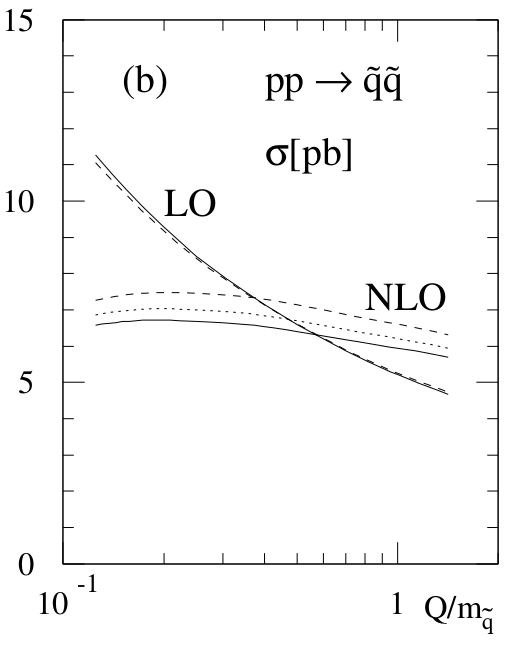
\includegraphics[scale=0.4]{squark_gluino_LO_NLO.png}
\caption{The dependence on the renormalization/factorization scale $Q$ of the LO and NLO cross sections for squark-squark production at the LHC ($\sqrt{s}=14$ TeV). Parton densities are GRV94 (solid), CTEQ3 (dashed) and MRS(A') (dotted). Mass parameters are $m_{\tilde{q}}=600$ GeV, $m_{\tilde{g}}=500$ GeV and $m_t=175$ GeV. Figure from \cite{beenakker1997squark}.}
\label{Fig:: hadron susy : LO vs NLO beenakker}
\end{figure}


The calculations from \cite{beenakker1997squark} assume degenerate squark masses $m_{\tilde{q}}$, set the 5 lightest quark masses to zero as they are much lighter than the squarks, and the top quark mass to $m_t =175$ GeV. The two free parameters left are then $m_{\tilde{g}}$ and $m_{\tilde{q}}$. This indicates that these might be good features for the learning. The renormalization scheme used is the $\bar{MS}$ scheme. Masses and couplings are renormalized, and the resulting parameters can be found in \cite{beenakker1997squark}.

\subsubsection{Partonic Cross-Section}

As previously discussed, calculations for hadron colliders require first finding the hadronic cross sections. In order to analyze these, scaling functions are introduced \cite{beenakker1997squark}
\begin{align}
\hat{\sigma}_{ij} = \frac{\alpha_s^2(Q^2)}{m^2} \Big\{ f^B_{ij}(\eta, r) + 4 \pi \alpha_s (Q^2) \Bigg[ f_{ij}^{V+S}(\eta, r, r_t) + f_{ij}^H (\eta, r) + \bar{f}_{ij} (\eta, r) \log \Bigg( \frac{Q^2}{m^2}\Bigg) \Bigg] \Big\}
,
\end{align}
where $Q^2$ is the mass scale, often set to $Q^2 = m^2$, and $m^2 = (\sqrt{p_1^2} + \sqrt{p_2^2})/2$ is the mass of the final particles. The scaling functions $f$ are divided as follows: the Born term $f^B$, the sum of virtual and soft-gluon corrections $f^{V+S}$, the hard gluon corrections $f^H$, and the scale-dependent contributions $\bar{f}$. The partonic cross section depends on the parameters
\begin{align}
&\eta = \frac{s}{4m^2} -1, &r= \frac{m_{\tilde{g}}^2}{m_{\tilde{q}}^2}, &&r_t = \frac{m_t^2}{m^2},
\end{align}
which may be used in deciding the target and features for the learning process.

\subsubsection{Hadronic Cross-Section}

As per the previous discussion, the partonic cross-sections must be integrated over in order to obtain the total hadronic cross section. A convolution integral over the parton distribution functions yields the expression 
\begin{align}
\sigma(S, Q^2) = \sum_{i,j=q, q, \bar{q}} \int_{\tau}^1dx_1 \int_{\tau/x_1}^1 dx_2 f_i^{h_1} (x_1, Q^2) f_j^{h_2}(x_2, Q^2) \hat{\sigma}_{ij} (x_!x_2S, Q^2)\Big|_{\tau=4m^2/S}.
\end{align}
The integrals are calculated numerically using the VEGAS integration routine \cite{PETERLEPAGE1978192} in \cite{beenakker1997squark}.
The uncertainty due to different parameterizations of the parton densities for the LHC calculations of the NLO terms amount to $\lesssim 13 \%$ at the central scale.

\subsubsection{K-Factor}

To quantify the improvement on the cross section found by adding NLO terms, the \textit{K-factor} is introduced. It is the ratio between the cross sections
\begin{align}
K = \sigma_{NLO}/\sigma_{LO}.
\end{align}
The $K$-factor for squark production for varying mass ratios $m_{\tilde{q}}/m_{\tilde{g}}=2.0, 1.6,1.2,0.8$ at the LHC is shown in Fig. (\ref{Fig:: susy hadron : K-factor LHC}). As seen from the figure, the $K$-factor is larger than 1 and quite stable as a function of the squark mass. This indicates a shift in the mass spectrum, and provides stronger bounds on particle masses.

\begin{figure}
\centering
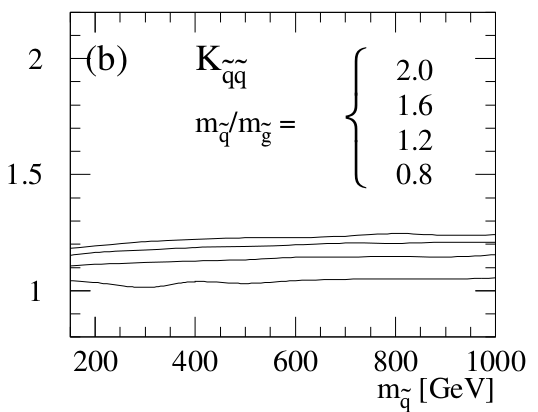
\includegraphics[scale=0.5]{squark_gluino_K_factor.png}
\caption{The $K$-factors for the LHC ($\sqrt{s}=14$ TeV). Parton densities are GRV94, with scale $Q=m$, and the top squark mass is $m_t=175$ GeV. Figure from \cite{beenakker1997squark}.}
\label{Fig:: susy hadron : K-factor LHC}
\end{figure}


\subsection{State-of-the-art Tools}

\subsubsection{Prospino}
A tool that uses the $K$-factor to calculate NLO cross sections is Prospino \cite{beenakker1996prospino}.

Trouble with Prospino for large masses, when $LO \neq 0$ and $NLO =0$. 


\subsubsection{NLL-fast}



\bibliographystyle{plain}
\bibliography{dingsen_susy_at_hadron_colliders}

\end{document}
